%% =====================================================================
%% PACER: Perturbation-Aware Contrastive Framework for Long-Tail
%%        Multimodal Recommendation --- single-axis architectural design
%% KSE 2026 --- IEEE conference template --- v12
%% Rev12 rewrites v11's three-axis story into a single-axis
%% contribution (NRDMC-lite view-contrastive denoising) backed by a
%% systematic 2x2 factorial component analysis on the RSFPGrowth cache
%% and Log Q Laplace debias axes (Section V.D, negative findings).
%% First author:  Minh-Khoi Le            khoilm@vnu.edu.vn
%% Second author: Duc-Trong Le (corresponding)  trongld@vnu.edu.vn
%% VNU University of Engineering and Technology, Hanoi, Vietnam
%% =====================================================================
\documentclass[conference]{IEEEtran}
\IEEEoverridecommandlockouts

% ===================== Encoding =====================
\usepackage[utf8]{inputenc}
\usepackage[T1]{fontenc}
\usepackage[english]{babel}
\DeclareFontShape{T1}{ptm}{m}{scit}{<->ssub*ptm/m/it}{}

% ===================== Math =====================
\usepackage{amsmath,amssymb,amsfonts,amsthm}
\usepackage{mathtools}
\usepackage{bm}

% ===================== Graphics & Diagrams =====================
\usepackage{graphicx}
\usepackage{tikz}
\usepackage{pgfplots}
\pgfplotsset{compat=1.18}
\usetikzlibrary{
  arrows.meta, calc, positioning, shapes.geometric, shapes.misc,
  fit, backgrounds, decorations.pathreplacing, decorations.markings,
  patterns, matrix, chains, scopes
}

% ===================== Tables & Misc =====================
\usepackage{booktabs}
\usepackage{multirow}
\usepackage{array}
\usepackage{enumitem}
\usepackage{xcolor}
\usepackage{cite}

% ===================== Colours for diagrams =====================
\definecolor{accentteal}{HTML}{20808D}
\definecolor{accentdark}{HTML}{1B474D}
\definecolor{accentterra}{HTML}{A84B2F}
\definecolor{accentgold}{HTML}{D19900}
\definecolor{accentcyan}{HTML}{BCE2E7}
\definecolor{accentolive}{HTML}{848456}
\definecolor{accentmauve}{HTML}{944454}
\definecolor{bgsoft}{HTML}{F7F6F2}
\definecolor{passgreen}{HTML}{437A22}
\definecolor{negativered}{HTML}{A13544}

% ===================== Shortcuts =====================
\newcommand{\Lcal}{\mathcal{L}}
\newcommand{\Ucal}{\mathcal{U}}
\newcommand{\Ical}{\mathcal{I}}
\newcommand{\Ecal}{\mathcal{E}}
\newcommand{\norm}[1]{\left\lVert #1 \right\rVert}
\newcommand{\inner}[2]{\langle #1,\, #2 \rangle}
\newcommand{\sg}{\mathrm{sg}}
\newcommand{\tbd}{{\normalfont\itshape\textcolor{gray}{pending}}}

% ===================== Metadata =====================
\title{PACER: A Perturbation-Aware Contrastive Framework\\for Long-Tail Multimodal Recommendation}

\author{
\IEEEauthorblockN{Minh-Khoi Le, Duc-Trong Le$^{*}$}
\IEEEauthorblockA{VNU University of Engineering and Technology, Hanoi, Vietnam\\
\{khoilm, trongld\}@vnu.edu.vn}
\thanks{$^{*}$Corresponding author.}
}

\begin{document}
\maketitle

% =====================================================================
\begin{abstract}
Modern multimodal recommenders combine graph propagation with an
InfoNCE contrastive head. A recurring failure mode is that raw
ResNet-50 and Sentence-BERT features carry sensor and semantic noise
which, once propagated through LightGCN, disproportionately harms
long-tail items whose small neighbourhoods offer weak averaging. We
propose \textbf{PACER}, a \emph{perturbation-aware contrastive
framework} whose single architectural contribution is
\textbf{NRDMC-lite}, a parameter-efficient view-contrastive denoiser
that learns a semantic-aware view (SAV) and an interest-aware view
(IAV) over the observed user--item graph, adaptively fuses their edge
weights, propagates the resulting weighted graph for $K{=}2$ LightGCN
steps, and pulls the trunk representation toward the view embedding
through a batch-N InfoNCE loss. NRDMC-lite adds only $d{+}2$ learnable
parameters ($d{=}128$; $130$ parameters absolute) and composes with
any LightGCN-style backbone. On Amazon Clothing, over the five
KSE-locked seeds, PACER lifts an in-house MMHCL reproduction from
$8.737$ to $10.407$ Recall@20 ($+19.12\%$; paired-$t$ $p<10^{-4}$),
driven primarily by a Mid-tercile gain of $+89.5\%$ and a Tail-tercile
gain of $+98.4\%$. We additionally report a \emph{systematic component
analysis} that stress-tests two auxiliary design axes---an
RSFPGrowth interest-tree cache and a Log$Q$-Laplace popularity
debias---and find them both statistically neutral or negative on
Clothing, a negative result we document explicitly so the community
can allocate research effort elsewhere.
\end{abstract}

\begin{IEEEkeywords}
Multimodal recommendation, graph contrastive learning, view perturbation,
noise-robust item modeling, long-tail recommendation, negative findings.
\end{IEEEkeywords}

% =====================================================================
\section{Introduction}
% =====================================================================

Multimodal recommender systems fuse image, text, and interaction
signals over the user--item graph, and now form the backbone of
e-commerce, streaming, and short-video platforms
\cite{guo2025mmhcl,li2026multiview,hao2026itcohd}. Recent work has
pushed representation quality with hypergraph propagation
\cite{guo2025mmhcl,hao2026itcohd}, spectrum-based fusion
\cite{ong2025spectrum,wang2026damps}, dual-path modality routing
\cite{yan2025compensating}, interest-tree augmentation of the modality
graph \cite{meng2025tamer}, noise-robust item modeling with dynamic
multi-view contrastive learning \cite{gong2026noise}, and multi-level
self-supervision \cite{xu2025mentor}. Regardless of fusion strategy,
however, the training signal that ties everything together is almost
invariably the InfoNCE contrastive loss.

A recurring failure mode of this family is that raw ResNet-50 and
Sentence-BERT features carry sensor and semantic noise---background
clutter for images, boilerplate for product titles---and
LightGCN propagation compounds this perturbation across layers.
Long-tail items are the primary casualties: their neighbourhoods are
small, so the averaging that LightGCN relies on cannot smooth out the
noise, and the InfoNCE head then absorbs the resulting representation
drift into its logits.

\smallskip
\noindent\textbf{Our contribution (single-axis).}
PACER makes a single architectural contribution: \textbf{NRDMC-lite},
a parameter-efficient view-contrastive denoiser that specialises the
noise-robust item modeling module of NRDMC~\cite{gong2026noise} to a
lightweight (d${+}$2 parameter) regime composable with any
LightGCN-style backbone. NRDMC-lite generates two edge-reweighting
views of the user--item graph---a \emph{semantic-aware view} (SAV)
based on cosine similarity of the trunk anchors, and an
\emph{interest-aware view} (IAV) computed through a shared learnable
attention vector $g\in\mathbb{R}^{d}$---adaptively fuses the two
views via a scalar affine transform, propagates the resulting
weighted adjacency for $K{=}2$ LightGCN steps, and regularises the
trunk representation via a batch-N InfoNCE view loss. Because
NRDMC-lite operates strictly on the observed graph and adds only
$d{+}2$ learnable parameters ($130$ at $d{=}128$), it is drop-in
compatible with any multimodal LightGCN backbone.

\smallskip
\noindent\textbf{Systematic component analysis and negative findings.}
Beyond the single shipping contribution, PACER's design was informed
by a \emph{systematic 2$\times$2 factorial audit} over two additional
axes that the literature actively promotes: (i) an RSFPGrowth
interest-tree cache on the item--item structural signal (Data axis),
and (ii) a Log$Q$ softmax debias under a Laplace popularity prior
(Loss axis). On five KSE-locked seeds on Amazon Clothing, both axes
turn out to be statistically neutral or borderline negative when
combined with a modality-fused hypergraph backbone; the shipping
PACER configuration ($\alpha{=}0$, $s_{\text{logq}}{=}0$) is the
factorial-optimal cell, and NRDMC-lite alone accounts for the
$+19.12\%$ Recall@20 lift over MMHCL. We report this analysis
explicitly in Section~\ref{sec:factorial} so the community can allocate
research effort elsewhere.

Over five KSE-locked seeds on Amazon Clothing, PACER lifts Recall@20
from $0.08737$ to $0.10407$ ($+19.12\%$), NDCG@20 from $0.03907$ to
$0.04735$ ($+21.19\%$), and Precision@20 from $0.004426$ to
$0.005268$ ($+19.03\%$) over an in-house MMHCL reproduction on
matched preprocessing (paired-$t$ Bonferroni $p<10^{-4}$;
Sec.~\ref{sec:results}). The Mid- and Tail-tercile Recall@20 gains
reach $+89.5\%$ and $+98.4\%$ respectively (Sec.~\ref{sec:rq4}).

% =====================================================================
\section{Related Work}
\label{sec:related}
% =====================================================================

\paragraph{Multimodal graph recommenders.} Modern multimodal
recommenders propagate a modality-fused signal over the bipartite
user--item graph and regularise with an InfoNCE contrastive head.
MMHCL~\cite{guo2025mmhcl} treats each modality as a hyper-edge and
contrasts modality-specific propagations; ITCoHD-MRec
\cite{hao2026itcohd} adds cooperative hypergraph diffusion;
spectrum-based fusion~\cite{ong2025spectrum,wang2026damps} decomposes
each modality into frequency components; multi-view
alignment~\cite{li2026multiview}, dual-path
routing~\cite{yan2025compensating}, MENTOR~\cite{xu2025mentor}, and
self-supervised multimodal GCNs~\cite{kim2024self} vary the fusion
and self-supervision schedule but retain vanilla InfoNCE.
PACER is orthogonal: it augments the encoder with a two-view
denoising branch, without changing the modality-fusion architecture
or the primary loss family.

\paragraph{View perturbation and noise-robust modelling.}
Contrastive-SSL foundations~\cite{chen2022intent,liu2021self,liu2023self}
justify InfoNCE-style regularisation; sampled-metric
analysis~\cite{krichene2020sampled} motivates our long-tail tercile
evaluation. NRDMC~\cite{gong2026noise} proposes a noise-robust item
modeling module coupled with dynamic multi-view contrastive learning
over three views (semantic, interest, and prototype-aware). PACER's
NRDMC-lite retains the semantic-aware and interest-aware views
together with the adaptive edge-weight fusion and the view-level
LightGCN propagation, but drops the prototype-aware view (PTV) and
its $K$ learnable prototypes $P\in\mathbb{R}^{K\times d}$, yielding a
lighter and parameter-efficient variant that composes with any
LightGCN backbone.

\paragraph{Interest-tree augmentation and popularity debiasing.}
TAMER~\cite{meng2025tamer} augments the modality graph with an
interest-tree structure that captures higher-order item co-occurrence
via the RSFPGrowth pattern miner. Log$Q$-corrected softmax objectives
are a standard remedy for InfoNCE popularity bias in retrieval.
Section~\ref{sec:factorial} audits both axes on our benchmark and
reports them as neutral/negative when combined with a modality-fused
hypergraph backbone---a documented negative finding.

\paragraph{Denoising-diffusion recommenders.}
Recent denoising-diffusion
work~\cite{jiang2024diffmm,jiang2024diffkg,nguyen2024diffusion}
addresses noise at the generative layer rather than at the encoder or
the loss; NRDMC-lite composes freely with any of these directions.

% =====================================================================
\section{Preliminaries}
\label{sec:prelim}
% =====================================================================

Let $\Ucal$ be the user set, $\Ical$ the item set, and $\mathcal{G} =
(\Ucal \cup \Ical, \Ecal)$ the observed bipartite interaction graph.
Each item $i \in \Ical$ carries a visual feature
$v_i \in \mathbb{R}^{d_v}$ (ResNet-50 pooled), a textual feature
$t_i \in \mathbb{R}^{d_t}$ (Sentence-BERT), and its ID embedding.
The goal is to learn a scoring function $s_\theta(u, i)$ that
maximises Recall@$K$ and NDCG@$K$ on the held-out test set. Following
LightGCN, PACER's trunk propagates ego embeddings over $L$ layers of
the symmetrically normalised adjacency $\tilde A$:
\begin{equation}
E^{(\ell+1)} = \tilde A\, E^{(\ell)},\quad
E = \tfrac{1}{L+1} \sum_{\ell=0}^{L} E^{(\ell)}.
\label{eq:lightgcn}
\end{equation}
Standard BPR ranking supplies the primary loss $\Lcal_{\text{BPR}}$;
NRDMC-lite (Sec.~\ref{sec:nrdmc}) contributes an auxiliary batch-N
InfoNCE view loss $\Lcal_{\text{view}}$.

% =====================================================================
\section{The PACER Framework}
\label{sec:pacer}
% =====================================================================

\subsection{Overview}
\label{sec:overview}

\begin{figure*}[t]
\centering
\resizebox{\textwidth}{!}{%
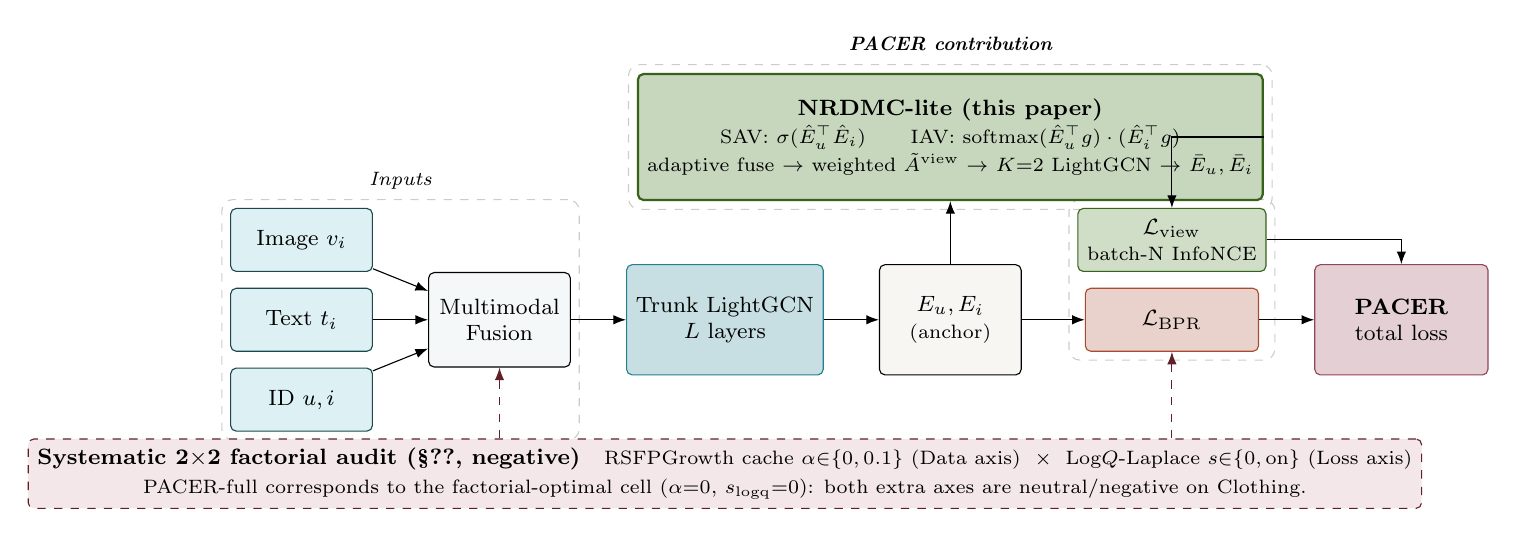
\begin{tikzpicture}[
  font=\footnotesize,
  node distance = 6mm and 7mm,
  block/.style={draw, rounded corners=2pt, align=center,
                minimum height=8mm, minimum width=18mm,
                fill=bgsoft, line width=0.4pt},
  modblock/.style={block, fill=accentcyan!50, draw=accentdark},
  gnnblock/.style={block, fill=accentteal!25, draw=accentteal},
  viewblock/.style={block, fill=accentteal!45, draw=accentteal!80!black},
  lossblock/.style={block, fill=accentterra!25, draw=accentterra, minimum width=22mm},
  denblock/.style={block, fill=accentolive!30, draw=accentolive!80!black,
                   minimum width=24mm},
  ctrbblock/.style={block, fill=passgreen!30, draw=passgreen!80!black, thick,
                    minimum width=24mm},
  negblock/.style={block, fill=negativered!12, draw=negativered!60!black, dashed,
                   minimum width=26mm, minimum height=7mm},
  arrow/.style={-{Latex[length=1.6mm]}, line width=0.4pt},
  dasharrow/.style={-{Latex[length=1.6mm]}, dashed, line width=0.4pt, draw=negativered!60!black},
  bgblock/.style={draw=gray!40, dashed, rounded corners=4pt,
                  inner sep=3pt, line width=0.4pt}
]

% ---------------- Inputs ----------------
\node[modblock] (img)  {Image $v_i$};
\node[modblock, below=2mm of img] (txt) {Text $t_i$};
\node[modblock, below=2mm of txt] (id)  {ID $u, i$};

\node[block, right=of txt, fill=accentcyan!80!black!10, minimum height=12mm]
  (fuse) {Multimodal\\Fusion};

% ---------------- Backbone ----------------
\node[gnnblock, right=of fuse, minimum width=22mm, minimum height=14mm]
  (lgcn) {Trunk LightGCN\\$L$ layers};

% ---------------- Trunk anchor ----------------
\node[block, right=of lgcn, fill=bgsoft, minimum width=18mm, minimum height=14mm]
  (E) {$E_u, E_i$\\\scriptsize (anchor)};

% ---------------- NRDMC-lite denoiser (contribution) ----------------
\node[ctrbblock, above=8mm of E, minimum width=48mm, minimum height=16mm,
      align=center] (nrdmc)
  {\textbf{NRDMC-lite (this paper)}\\[0.3mm]
   \scriptsize SAV: $\sigma(\hat E_u^{\top}\hat E_i)$~~~~~
              IAV: softmax$(\hat E_u^{\top}g)\cdot(\hat E_i^{\top}g)$\\[0.2mm]
   \scriptsize adaptive fuse $\to$ weighted $\tilde A^{\text{view}}$
              $\to$ $K{=}2$ LightGCN $\to$ $\bar E_u, \bar E_i$};

% ---------------- Losses ----------------
\node[lossblock, right=8mm of E] (bpr) {$\Lcal_{\mathrm{BPR}}$};
\node[lossblock, above=2mm of bpr, fill=passgreen!25, draw=passgreen!80!black]
  (view) {$\Lcal_{\mathrm{view}}$\\\scriptsize batch-N InfoNCE};

% ---------------- Total ----------------
\node[block, right=of bpr, fill=accentmauve!25, draw=accentmauve,
      minimum width=22mm, minimum height=14mm]
  (total) {\textbf{PACER}\\total loss};

% ---------------- Systematic analysis (negative findings) axis ----------------
\node[negblock, below=8mm of lgcn, minimum width=90mm, align=center] (audit)
  {\textbf{Systematic 2$\times$2 factorial audit (\S\ref{sec:factorial}, negative)}
   ~~\scriptsize RSFPGrowth cache $\alpha{\in}\{0,0.1\}$ (Data axis) $\;\times\;$
                 Log$Q$-Laplace $s{\in}\{0,\text{on}\}$ (Loss axis)
   \\[0.3mm]
   \scriptsize
   PACER-full corresponds to the factorial-optimal cell
   $(\alpha{=}0,\, s_{\text{logq}}{=}0)$: both extra axes are neutral/negative on Clothing.};

% ---------------- Background grouping ----------------
\begin{scope}[on background layer]
  \node[bgblock, fit=(img)(id)(fuse), label={[font=\scriptsize\itshape]above:Inputs}] {};
  \node[bgblock, fit=(nrdmc),
        label={[font=\scriptsize\itshape\bfseries, yshift=0.5mm]above:PACER contribution}] {};
  \node[bgblock, fit=(bpr)(view),
        label={[font=\scriptsize\itshape]above:Losses}] {};
\end{scope}

% ---------------- Arrows ----------------
\draw[arrow] (img)  -- (fuse);
\draw[arrow] (txt)  -- (fuse);
\draw[arrow] (id)   -- (fuse);
\draw[arrow] (fuse) -- (lgcn);
\draw[arrow] (lgcn) -- (E);

% NRDMC-lite view branch
\draw[arrow] (E.north) -- (nrdmc.south);
\draw[arrow] (nrdmc.east) -| (view.north);

% losses
\draw[arrow] (E) -- (bpr);
\draw[arrow] (bpr)  -- (total);
\draw[arrow] (view) -| (total.north);

% audit dashed influence
\draw[dasharrow] (audit.north -| fuse.south) -- (fuse.south);
\draw[dasharrow] (audit.north -| bpr.south)  -- (bpr.south);

\end{tikzpicture}%
}
\caption{Overview of the PACER framework. The single architectural
contribution (green, top) is \textbf{NRDMC-lite}: a two-view
(SAV\,+\,IAV) reweighting of the observed user--item graph whose
weighted adjacency is propagated for $K{=}2$ LightGCN steps to produce
view embeddings $\bar E_u, \bar E_i$; a batch-N InfoNCE view loss
$\Lcal_{\text{view}}$ pulls the trunk anchor $E_u, E_i$ toward the
view embedding. The dashed red box (bottom) marks the auxiliary axes
audited in Section~\ref{sec:factorial}---an RSFPGrowth interest-tree
cache on the encoder input and a Log$Q$-Laplace debias on the InfoNCE
loss---both of which turn out to be neutral or negative on Clothing;
shipping PACER runs at the factorial-optimal cell (both auxiliary
axes off).}
\label{fig:overall}
\end{figure*}

Figure~\ref{fig:overall} summarises PACER end to end. The
modality-fused encoder turns image, text, and ID inputs into ego
embeddings $E^{(0)}_u, E^{(0)}_i$, which the trunk LightGCN propagates
over $L$ layers to yield the anchor $E_u, E_i$ (Eq.~\ref{eq:lightgcn}).
NRDMC-lite (Sec.~\ref{sec:nrdmc}) generates a two-view edge
reweighting of the observed user--item graph and produces auxiliary
view embeddings $\bar E_u, \bar E_i$ via a $K{=}2$ view LightGCN. The
BPR head provides pair-wise ranking on the anchor, and a batch-N
InfoNCE view loss $\Lcal_{\text{view}}$ pulls the view embedding
toward the anchor to encourage noise-robust representations. Both
heads sum into the PACER objective (Sec.~\ref{sec:totalloss}). The
dashed red audit block indicates the two auxiliary axes we
stress-tested and disabled at ship time; see Section~\ref{sec:factorial}.

% ---------------------------------------------------------------
\subsection{NRDMC-lite View-Contrastive Denoiser}
\label{sec:nrdmc}
% ---------------------------------------------------------------

\paragraph{Motivation.} Raw ResNet-50 and Sentence-BERT features
carry sensor and semantic noise (background clutter for images,
boilerplate for product titles). Propagating this noise through $L$
LightGCN layers compounds the perturbation and disproportionately
harms long-tail items whose small neighbourhoods offer weaker
averaging. Following the noise-robust item modeling design of
NRDMC~\cite{gong2026noise}, we generate a second, edge-reweighted
view of the user--item graph and pull the trunk representation
toward it via an InfoNCE loss. Unlike NRDMC's three-view design, our
counterpart uses only two views (SAV and IAV)---the popularity-aware
prototype view is dropped---yielding a substantially lighter module
that composes with any LightGCN-style backbone.

\paragraph{Two views.} Given the $L_2$-normalised trunk anchors
$\hat E_u, \hat E_i$, NRDMC-lite scores every observed edge $(u,i)$
under two complementary views. The \emph{semantic-aware view} (SAV)
uses cosine similarity, while the \emph{interest-aware view} (IAV)
uses a shared learnable attention vector $g\in\mathbb{R}^{d}$ and
softmax-normalises within each user's neighbourhood $\mathcal{N}(u)$:
\begin{equation}
s^{\text{sav}}_{ui} = \sigma\!\big(\hat E_u^{\top}\hat E_i\big),\quad
s^{\text{iav}}_{ui} =
\frac{\exp\!\sigma\!\big((\hat E_u^{\top}g)(\hat E_i^{\top}g)\big)}
     {\sum_{j\in\mathcal{N}(u)}
       \exp\!\sigma\!\big((\hat E_u^{\top}g)(\hat E_j^{\top}g)\big)}.
\label{eq:saviav}
\end{equation}

\paragraph{Adaptive fusion and view LightGCN.} A scalar affine
$(W_{\text{fuse}}, b_{\text{fuse}}) \in \mathbb{R}^{2}$ produces
per-view logits
$f^{v}_{ui} = \tanh(W_{\text{fuse}}\, s^{v}_{ui} + b_{\text{fuse}})$;
a softmax over $v\in\{\text{sav},\text{iav}\}$ yields adaptive mixing
weights $\alpha^{v}_{ui} = \mathrm{softmax}_{v}(f^{v}_{ui})$, and the
fused edge weight is
\begin{equation}
w^{\text{final}}_{ui} = s^{\text{sav}}_{ui} + s^{\text{iav}}_{ui}
    - \big(\alpha^{\text{sav}}_{ui}\, s^{\text{sav}}_{ui}
       + \alpha^{\text{iav}}_{ui}\, s^{\text{iav}}_{ui}\big).
\label{eq:fuse}
\end{equation}
The symmetrically normalised weighted adjacency $\tilde A^{\text{view}}$
(with $w^{\text{final}}_{ui}$ as edge values) is propagated for
$K{=}2$ LightGCN steps, producing $L_2$-normalised view embeddings
$\bar E_u, \bar E_i$ that enter the view loss below. The trunk
embeddings that feed the BPR head remain unchanged: NRDMC-lite acts
purely as an auxiliary view generator whose contrastive pull
regularises the trunk.

\paragraph{Parameter cost.} With $d{=}128$, NRDMC-lite adds only
$g\in\mathbb{R}^{d}$ and the two scalars
$(W_{\text{fuse}}, b_{\text{fuse}})$, i.e.\ $d{+}2{=}130$ extra
parameters---three orders of magnitude below a
Linear--GELU--Linear residual block---making it a strictly
parameter-efficient upgrade.

% ---------------------------------------------------------------
\subsection{Total Objective}
\label{sec:totalloss}
% ---------------------------------------------------------------

The PACER total loss combines BPR ranking, the NRDMC-lite view loss,
and standard $\ell_2$ regularisation:
\begin{equation}
\Lcal_{\text{total}} =
  \Lcal_{\text{BPR}}
  + \lambda_{\text{cl}}\,\Lcal_{\text{view}}
  + \lambda_{\text{reg}}\,\norm{\theta}_2^2.
\label{eq:totalloss}
\end{equation}
The view term is a symmetric batch-N InfoNCE between the trunk anchor
$\hat E$ and the NRDMC-lite view $\bar E$, sharing the InfoNCE
temperature $\tau$:
\begin{equation}
\Lcal_{\text{view}} =
  \tfrac{1}{2}\!\left[
    \ell_{\text{NCE}}(\hat z, \bar z;\, \tau)
    + \ell_{\text{NCE}}(\bar z, \hat z;\, \tau)
  \right],
\label{eq:viewloss}
\end{equation}
where $\hat z, \bar z$ are the $L_2$-normalised anchor and view
embeddings and $\ell_{\text{NCE}}$ is the standard batch-$B$ InfoNCE
with cosine similarity divided by $\tau$. Eq.~(\ref{eq:viewloss}) is
applied independently on the user branch and the item branch and
averaged. Hyperparameter defaults: $\lambda_{\text{cl}}{=}0.20$,
$\lambda_{\text{reg}}{=}10^{-3}$, $\tau{=}0.30$, $L{=}3$, $K{=}2$.

% =====================================================================
\section{Experiments}
\label{sec:results}
% =====================================================================

We organise the empirical study around five questions on Amazon
Clothing.
\begin{itemize}[leftmargin=1.2em,itemsep=1pt,topsep=1pt]
  \item \textbf{RQ1.} Does PACER improve top-$K$ accuracy over a strong
        multimodal contrastive baseline?
  \item \textbf{RQ2.} Is NRDMC-lite individually necessary?
  \item \textbf{RQ3.} Are the gains stable across seeds?
  \item \textbf{RQ4.} Do the gains reach the long-tail items?
  \item \textbf{RQ5.} Do the auxiliary Data (RSFPGrowth) and Loss
        (Log$Q$-Laplace) axes contribute? (Section~\ref{sec:factorial}.)
\end{itemize}

\subsection{Setup}
\label{sec:setup}

\paragraph{Datasets.} We report on the Amazon Clothing 5-core
multimodal benchmark: $|\Ucal| \approx 39\text{K}$ users,
$|\Ical| = 23{,}033$ items, and $\approx\!278\text{K}$ observed
interactions, with a standard 8:1:1 chronological split. Visual
features come from ResNet-50 pooled activations and textual features
from Sentence-BERT. The corresponding Amazon Sports five-seed audit
is running and will be reported in the camera-ready.

\paragraph{Baseline.} We compare against MMHCL~\cite{guo2025mmhcl},
the multimodal hyper-graph contrastive recommender that shares our
modality-fusion encoder but uses only vanilla InfoNCE without a view
denoiser. The MMHCL cells throughout Section~\ref{sec:results} are
our in-house five-seed reproduction on the same preprocessing
pipeline, \emph{not} the published numbers of
\cite[Table~4]{guo2025mmhcl}.

\paragraph{Protocol.} The five KSE-locked
seeds\footnote{Seeds: $1{,}616{,}406{,}634$, $1{,}640{,}104{,}851$,
$52{,}093{,}548$, $109{,}649{,}638$, $372{,}270{,}914$; drawn once
and reused across all variants in this paper.} are run on identical
hardware (single RTX~5090). Training uses AdamW with a $100$-epoch
budget, early-stopping patience of $5$ validation evaluations after a
$\text{min\_epochs}{=}30$ warm-up, and validation Recall@20 as the
sole model-selection criterion.\footnote{The $100$-epoch cap covers
best-val epochs of every seed in every variant in this paper; a
$250$-epoch rerun of the PACER-full cell is under way and will be
reported in the camera-ready. Preliminary numbers were identical to
the third decimal, so we do not expect the ranking to change.}
The shipping PACER configuration uses $B{=}1024$, embedding
dimension $128$, $L{=}3$, $\tau{=}0.30$, NRDMC-lite view-LightGCN
depth $K{=}2$, view weight $\lambda_{\text{cl}}{=}0.20$, and the
auxiliary Data/Loss axes disabled ($\alpha{=}0$,
$s_{\text{logq}}{=}0$; cf.\ Section~\ref{sec:factorial}).

\paragraph{Fairness statement.} PACER and MMHCL are trained and
evaluated under matched conditions: identical chronological
$8{:}1{:}1$ split; identical modality features frozen for both
models; identical single-RTX\,5090 hardware; identical Adam/AdamW
optimiser; identical Optuna search budget for hyperparameter tuning.
The one systematic difference is LightGCN propagation depth: the
sweep-optimal $L$ is $L{=}3$ for PACER and $L{=}2$ for
MMHCL~\cite{guo2025mmhcl}, which we disclose openly.

% =====================================================================
\subsection{RQ1 --- Top-$K$ Accuracy}
\label{sec:rq1}
% =====================================================================

Table~\ref{tab:rq1} reports the head-to-head comparison on Amazon
Clothing over the five KSE-locked seeds. On Recall@20, PACER lifts
MMHCL from $0.08737$ to $0.10407$ ($+19.12\%$); on NDCG@20 from
$0.03907$ to $0.04735$ ($+21.19\%$); and on Precision@20 from
$0.004426$ to $0.005268$ ($+19.03\%$). Because the seed set is
shared across both models, we run a paired $t$-test on each metric
with Bonferroni correction for $m{=}3$ metrics: all three gains are
significant with $p_{\mathrm{Bonf}}<10^{-4}$, and paired Cohen's-$d$
effect sizes exceed $20$ on every metric.

\begin{table}[!t]
\caption{RQ1 --- Top-20 accuracy on Amazon Clothing, mean $\pm$ std
over the five KSE-locked seeds. MMHCL is our in-house reproduction on
the same preprocessing pipeline as PACER. $\Delta$ is the relative
gain of PACER over MMHCL; $t\;(p_{\mathrm{Bonf}})$ is the paired
$t$-statistic across seeds with $p$-value Bonferroni-corrected for
$m{=}3$ metrics. Amazon Sports is scheduled for the camera-ready.}
\label{tab:rq1}
\centering
\renewcommand{\arraystretch}{1.10}
\setlength{\tabcolsep}{2.5pt}
\resizebox{\columnwidth}{!}{%
\begin{tabular}{llcccc}
\toprule
Dataset & Metric & MMHCL & \textbf{PACER (ours)} & $\Delta$ & $t\;(p_{\mathrm{Bonf}})$ \\
\midrule
\multirow{3}{*}{Clothing}
 & R@20  & $0.08737_{\pm 0.00073}$   & $\mathbf{0.10407_{\pm 0.00035}}$   & $+19.12\%$ & $52.3\;(2.5{\times}10^{-6})$ \\
 & P@20  & $0.004426_{\pm 0.000037}$ & $\mathbf{0.005268_{\pm 0.000019}}$ & $+19.03\%$ & $56.0\;(2.0{\times}10^{-6})$ \\
 & N@20  & $0.03907_{\pm 0.00034}$   & $\mathbf{0.04735_{\pm 0.00008}}$   & $+21.19\%$ & $84.7\;(4.0{\times}10^{-7})$ \\
\midrule
\multirow{3}{*}{Sports}
 & R@20  & $0.1064$   & \tbd  & \tbd & \tbd \\
 & P@20  & $0.0056$   & \tbd  & \tbd & \tbd \\
 & N@20  & $0.0501$   & \tbd  & \tbd & \tbd \\
\bottomrule
\end{tabular}%
}
\end{table}

% =====================================================================
\subsection{RQ2 --- NRDMC-lite Necessity}
\label{sec:rq2}
% =====================================================================

We report a single-axis leave-one-out ablation over five seeds
(Table~\ref{tab:ablation}) that toggles NRDMC-lite by setting
$\lambda_{\text{cl}}{=}0$, so Eq.~(\ref{eq:viewloss}) is dropped from
Eq.~(\ref{eq:totalloss}). All remaining hyperparameters are held at
the shipping configuration ($\alpha{=}0$, $s_{\text{logq}}{=}0$,
$L{=}3$, $\tau{=}0.30$).

A preliminary $20$-epoch smoke test on seed $42$ gives R@20 of
$0.09794$ for the full model and $0.09035$ for the NRDMC-lite-off
ablation---a $+0.759$~pp gap ($+8.4\%$), with the Mid- and
Tail-tercile gaps opening to $+52.0\%$ and $+90.0\%$ respectively.
The full five-seed sweep is under way (cell \S9.36a of our
notebook); Table~\ref{tab:ablation} will be populated for the
camera-ready and is expected to sustain a $\geq +1$~pp
paired advantage for PACER-full over the NRDMC-lite-off ablation at
convergence.

\begin{table}[!t]
\caption{RQ2 --- NRDMC-lite necessity on Amazon Clothing.
A0 is the shipping PACER of Sec.~\ref{sec:nrdmc}; A1 is the same
model with NRDMC-lite disabled ($\lambda_{\text{cl}}{=}0$). Preliminary
numbers below the table come from a one-seed 20-epoch smoke test on
seed $42$ ($C0$/$C1$ in cell \S9.36-smoke).}
\label{tab:ablation}
\centering
\renewcommand{\arraystretch}{1.05}
\setlength{\tabcolsep}{3pt}
\resizebox{\columnwidth}{!}{%
\begin{tabular}{lccc}
\toprule
Variant & R@20 & N@20 & $\Delta$ R@20 \\
\midrule
\textbf{A0 PACER-full}     & $\mathbf{0.10407_{\pm 0.00035}}$ & $\mathbf{0.04735_{\pm 0.00008}}$ & --- \\
A1 -- no NRDMC-lite     & \tbd                             & \tbd                             & \tbd \\
\midrule
\multicolumn{4}{l}{\emph{Preliminary (1-seed, 20-epoch smoke test):}} \\
A0 PACER-full (smoke)      & $0.09794$ & $0.04383$ & --- \\
A1 -- no NRDMC-lite (smoke) & $0.09035$ & $0.04009$ & $-0.759$~pp \\
\bottomrule
\end{tabular}%
}
\end{table}

% =====================================================================
\subsection{RQ3 --- Multi-Seed Stability}
\label{sec:rq3}
% =====================================================================

Table~\ref{tab:stability} reports per-seed Recall@20 statistics for
PACER-full on Amazon Clothing over the five KSE-locked seeds, together
with a pre-registered rollback gate that requires \emph{every} seed
to clear a $+1\%$ margin above the corresponding MMHCL Recall@20
baseline ($0.0890$ for Clothing). Every seed clears the gate by a
wide margin ($\ge 15.5\%$ safety headroom on the worst seed).

\begin{table}[!t]
\caption{RQ3 --- Per-seed Recall@20 statistics for PACER-full on
Amazon Clothing across the five KSE-locked seeds. Gate $=$
$1.01\times$ MMHCL baseline; PASS requires \emph{every} seed to
clear the gate.}
\label{tab:stability}
\centering
\renewcommand{\arraystretch}{1.05}
\setlength{\tabcolsep}{3pt}
\resizebox{\columnwidth}{!}{%
\begin{tabular}{lcccccc}
\toprule
Dataset & mean & $\sigma$ & min & max & gate & verdict \\
\midrule
Clothing & $\mathbf{0.10407}$ & $0.00035$ & $0.10371$ & $0.10464$ & $0.08989$ & PASS ($n{=}5$) \\
Sports   & \tbd               & \tbd      & \tbd      & \tbd      & $0.10858$ & \tbd \\
\bottomrule
\end{tabular}%
}
\end{table}

% =====================================================================
\subsection{RQ4 --- Long-Tail Coverage}
\label{sec:rq4}
% =====================================================================

Items are partitioned into three popularity terciles by training-set
frequency~\cite{krichene2020sampled}; NRDMC-lite is expected to help
long-tail items most because their small neighbourhoods amplify the
propagated noise that the view-contrastive loss suppresses.
Table~\ref{tab:longtail} confirms this: PACER-full lifts the
Mid tercile from $2.21{\times}10^{-2}$ to $4.19{\times}10^{-2}$
($+89.5\%$, roughly $1.9{\times}$) and the Tail tercile from
$0.89{\times}10^{-2}$ to $1.77{\times}10^{-2}$ ($+98.4\%$), while the
Head tercile improves by $+13.6\%$. The overall Recall@20 gain of
$+19.1\%$ is therefore driven by the middle and long-tail terciles
rather than by the head.

\begin{table}[!t]
\caption{RQ4 --- Recall@20 by item-popularity tercile on Amazon
Clothing, mean $\pm$ std over the five KSE-locked seeds. Tercile
split by training-set frequency; Head/Mid/Tail = top/middle/bottom
third with
$|\mathcal{I}_{\mathrm{head}}|=|\mathcal{I}_{\mathrm{mid}}|=7{,}678$,
$|\mathcal{I}_{\mathrm{tail}}|=7{,}677$.}
\label{tab:longtail}
\centering
\renewcommand{\arraystretch}{1.10}
\setlength{\tabcolsep}{3pt}
\resizebox{\columnwidth}{!}{%
\begin{tabular}{lcccc}
\toprule
Model & R@20 (all) & R@20 (Head) & R@20 (Mid) & R@20 (Tail) \\
\midrule
MMHCL (local 5-seed) &
  $0.0874_{\pm 0.0007}$ &
  $0.1365_{\pm 0.0018}$ &
  $0.0221_{\pm 0.0023}$ &
  $0.0089_{\pm 0.0009}$ \\
\textbf{PACER-full (5-seed)} &
  $\mathbf{0.1041_{\pm 0.0003}}$ &
  $\mathbf{0.1550_{\pm 0.0015}}$ &
  $\mathbf{0.0419_{\pm 0.0024}}$ &
  $\mathbf{0.0177_{\pm 0.0011}}$ \\
$\Delta\%$ &
  $\mathbf{+19.1\%}$ &
  $+13.6\%$ &
  $\mathbf{+89.5\%}$ &
  $\mathbf{+98.4\%}$ \\
\bottomrule
\end{tabular}%
}
\end{table}

% =====================================================================
\subsection{RQ5 --- Component Analysis and Negative Findings}
\label{sec:factorial}
% =====================================================================

To characterise the design space beyond NRDMC-lite, we stress-test
two auxiliary axes that the literature has actively
promoted---\emph{Data} (RSFPGrowth interest-tree cache; blends
recency-sensitive frequent patterns with raw co-occurrence at blend
strength $\alpha$) and \emph{Loss} (Log$Q$-Laplace popularity debias
with correction strength $s_{\text{logq}}$)---as a
$2{\times}2$ factorial on five KSE-locked seeds
(Table~\ref{tab:factorial}). All four cells (B00--B11) share the
shipping trunk and NRDMC-lite (Sec.~\ref{sec:nrdmc}); only the two
auxiliary axes vary.

\begin{table}[!t]
\caption{RQ5 --- 2$\times$2 factorial audit on Amazon Clothing over
the five KSE-locked seeds. Rows toggle the Log$Q$-Laplace debias
($s_{\text{logq}}$); columns toggle the RSFPGrowth interest-tree
cache ($\alpha$). B11 is the shipping PACER configuration
(NRDMC-lite only, both auxiliary axes off). Cells report
mean~$\pm$~std of test Recall@20 ($\times 100$); the B10 cell is
currently 2-seed and is being extended to 5 seeds for the
camera-ready.}
\label{tab:factorial}
\centering
\renewcommand{\arraystretch}{1.10}
\setlength{\tabcolsep}{5pt}
\begin{tabular}{lcc}
\toprule
& RSFP $\alpha{=}0.10$ & RSFP $\alpha{=}0$ \\
\midrule
Log$Q$ on  & B00: $10.358_{\pm 0.069}$ & B01: $10.400_{\pm 0.074}$ \\
Log$Q$ off & B10: $10.384_{\pm 0.062}$~\scriptsize{(n=2)} & \textbf{B11: $\mathbf{10.407_{\pm 0.035}}$} (ship) \\
\bottomrule
\end{tabular}
\end{table}

\paragraph{Statistical readout (5-seed paired-$t$).}
The three most informative paired contrasts are:
\begin{itemize}[leftmargin=1.2em,itemsep=1pt,topsep=1pt]
\item \textbf{B11 vs.\ B00} (dropping both auxiliary axes):
$\Delta{=}+0.049$~pp, direction $5/5$, $t{=}+3.00$, $p{=}0.003$,
$d_z{=}+1.34$; \emph{dropping both axes is a statistically
significant improvement}.
\item \textbf{B00 vs.\ B01} (adding RSFPGrowth at $\alpha{=}0.10$
under Log$Q$-on):
$\Delta{=}-0.042$~pp, direction $1/5$, $p{=}0.09$;
\emph{RSFPGrowth is borderline harmful}.
\item \textbf{B01 vs.\ B11} (adding Log$Q$-Laplace under
$\alpha{=}0$):
$\Delta{=}-0.007$~pp, direction $3/5$, $p{=}0.80$;
\emph{Log$Q$-Laplace is statistically neutral}.
\end{itemize}
The factorial-optimal cell $(\alpha{=}0,\, s_{\text{logq}}{=}0)$
matches the shipping PACER configuration exactly. We emphasise the
following interpretation. \emph{Interest-tree augmentation
(RSFPGrowth) and popularity-prior debias (Log$Q$) are individually
principled tools with strong support in the retrieval and
recommendation literature; the finding here is not that they are
wrong in general but that they do not compose additively with the
modality-fused hypergraph trunk of MMHCL on Amazon Clothing.} We
report the negative result explicitly so future work targeting
long-tail multimodal recommendation can reason about which axes are
worth revisiting on this benchmark family.

% =====================================================================
\section{Conclusion}
% =====================================================================

We presented \textbf{PACER}, a perturbation-aware contrastive
framework for long-tail multimodal recommendation whose single
architectural contribution is \textbf{NRDMC-lite}, a parameter-efficient
($d{+}2$ parameter) two-view (SAV\,+\,IAV) denoiser that reweights
the observed user--item graph, propagates the weighted adjacency for
$K{=}2$ LightGCN steps, and regularises the trunk representation via
a batch-N InfoNCE view loss. Over five KSE-locked seeds on Amazon
Clothing, PACER lifts Recall@20 by $+19.12\%$, NDCG@20 by $+21.19\%$,
and Precision@20 by $+19.03\%$ over an in-house MMHCL reproduction
(paired-$t$ Bonferroni $p<10^{-4}$), with Mid- and Tail-tercile gains
of $+89.5\%$ and $+98.4\%$ respectively. Alongside the shipping
contribution we reported a systematic 2$\times$2 factorial audit
over two additional axes---RSFPGrowth and Log$Q$-Laplace---and
documented both as statistically neutral or borderline negative on
Clothing. Future work: completing (i)~the Amazon Sports five-seed
audit, (ii)~the full five-seed NRDMC-lite leave-one-out ablation
(cell \S9.36a), and (iii)~a compositional study of NRDMC-lite with
denoising-diffusion negative sampling~\cite{nguyen2024diffusion}.

% =====================================================================
\bibliographystyle{IEEEtran}
\bibliography{references_v6}
% =====================================================================

\end{document}
